\subsection{Industry adoption}

Despite all the prophecies of doom, functional programming can be considered an elementary part of today's IT landscape. Already more than 20 years ago Wadler presented "an angry half-dozen" examples of functional programming use cases in the real world (\cite[25]{wadler_functional_1997}). For example, Erlang, which is today seen as one of the fundamental building blocks of applications serving billions of users every day (\cite{reed_thats_2014}). However, despite those examples of successful application, in comparison to other paradigms and especially OOP, functional programming is still not a mainstream paradigm.

\begin{table}[H]
\centering
\caption{Programming Language Adoption and Perception}
\label{table:languageadoption}
\begin{tabular*}{\textwidth}{@{\extracolsep{\fill}} lllrrrr}
\toprule
Language    & Platform\tablefootnote{Apple: macOS, iOS, iPadOS, watchOS.} & Type\tablefootnote{Most of the languages listed here are in fact multi-paradigm languages which offer both functional and object-oriented capabilities. The type in this context refers to how those languages are mainly used.} & \multicolumn{1}{r}{Used\tablefootnote{By professional developers.}} & \multicolumn{1}{r}{Loved\tablefootnote{Developers want to continue to work with these languages.}} & \multicolumn{1}{r}{Dreaded\tablefootnote{Developers do not express interest in continuing to work with these languages.}} & \multicolumn{1}{r}{Wanted\tablefootnote{Developers do not yet use these languages, but want to learn them.}} \\ \midrule
C\#         & .NET     & OOP  & 31.9\%                          & 67.0\%                         & 33.0\%                           & 7.0\%                           \\
F\#         & .NET     & FP   & n/a                             & 61.7\%                         & 38.3\%                           & 3.3\%                           \\ \midrule
Java        & JVM      & OOP  & 39.2\%                          & 53.4\%                         & 46.6\%                           & 8.3\%                           \\
Kotlin      & JVM      & OOP   & 6.6\%                           & 72.6\%                         & 27.4\%                           & 11.1\%                          \\
Clojure     & JVM      & FP   & 1.5\%                           & 68.3\%                         & 31.7\%                           & 2.2\%                           \\
Scala       & JVM      & FP   & 4.2\%                           & 58.3\%                         & 41.7\%                           & 4.3\%                           \\ \midrule
Objective-C & Apple   & OOP  & 5.2\%                           & n/a                            & 68.7\%                           & n/a                             \\
Swift       & Apple    & OOP   & 6.8\%                           & 69.2\%                         & 30.8\%                           & 5.8\%                           \\ \bottomrule
\end{tabular*}
\tablesource{Own illustration based on \cite{stack_overflow_annual_2019}}
\end{table}

If one thing gets clear from the numbers presented in table \ref{table:languageadoption}, then that traditional and well-established languages like Java and C\# still dominate their respective platforms. The exception here is Swift. Considering its young age (it was published in 2014), this seems surprising at first. However, looking at how discontent programmers are with Objective-C, not so much anymore. Not even the immaturity of the tooling around the language like its IDE Xcode (\cite{reboucas_empirical_2016}) could stop the migration.

So why are most of the young contenders stuck with little recognition in their niches, while Swift is taking off so quickly? \cite{sink_why_2015} predicted Swift's success precisely while writing about why F\# is not making ground against C\#. He based his explanation on the theory of "The Chasm" by Geoffrey A. Moore, first published in the book "Crossing the Chasm" (\cite{moore_crossing_1991}).

\begin{figure}[h]
\centering
\caption{The Revised Technology Adaption Life Cycle}
\label{fig:chasm}
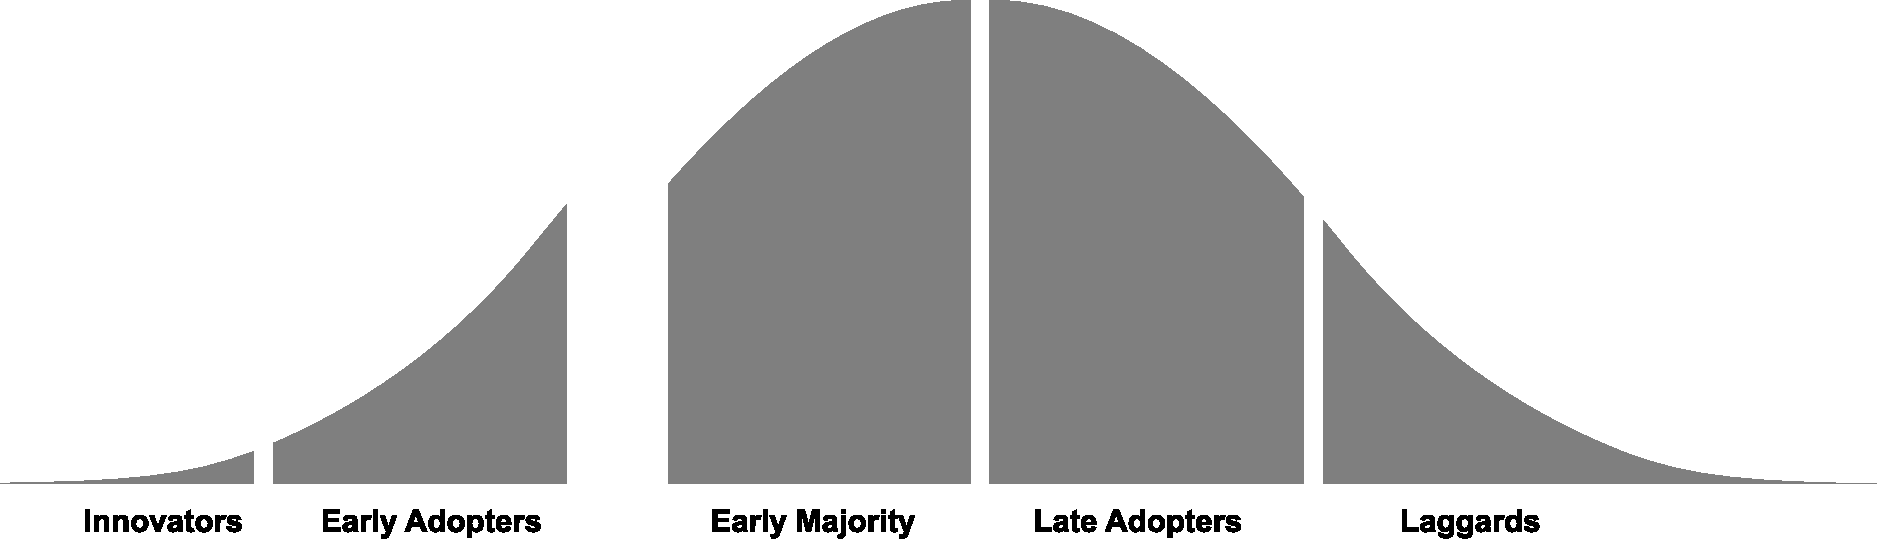
\includegraphics[width=\textwidth]{chasm}
\source{Own illustration based on \cite[13]{moore_crossing_1991}}
\end{figure}

The chasm describes the gap of adoption between the group of early adopters and the majority of users. While early adopters may accept some problems on the way (like immature tooling), the majority expects a definite productivity improvement without disrupting the way they work (evolution instead of revolution). Sink concludes that it needs severe problems to tackle and massive discontent with existing solutions in order to accept new approaches by the majority, which for those approaches then means "to cross the chasm."

For developers building applications in the Apple ecosystem, the primary hard problem seems to be Objective-C. In other words, "the pain" is so significant that developers were almost desperately waiting for an alternative language and are now happily joining the movement of the Swift language.

How about the JVM and .NET? Java did evolve relatively slowly over the last years compared to C\#, which early on got features like Generics (\cite{kennedy_design_2001}), LINQ (\cite{meijer_linq:_2006}), and async/await (\cite{hejlsberg_introducing_2010}). That may have made some room for improvement brought by new languages like Clojure and Scala, and especially Kotlin. Also, as seen in table \ref{table:languageadoption}, all three Java contenders are more appreciated than Java is itself within the JVM community. Interestingly, the opposite seems to be the case for .NET: F\# programmers love their language, but so do C\# programmers. Which may explain the low adoption rate of F\# compared to C\#. 

What could be done to make functional programming attractive for a broader audience? \cite[23]{wadler_why_1998} lists several factors that a functional language must support in order to attract people to adopt it on a larger scale: "To be widely used, a language should support interlanguage working, possess extensive libraries, be highly portable, have a stable and easy to install implementation, come with debuggers and profilers, be accompanied by training courses, and have a good track record on previous projects." The first five of those factors, which are mainly technical, are provided by almost all of the functional languages. 

Training, as the sixth factor, is indeed a problem not to be underestimated. As \cite[86]{hinsen_promises_2009} notes, "functional programming is very different from traditional programming \dots\ and thus requires a lot of learning and unlearning." However, as some of the functional languages and architectures become more and more widespread, a lot of learning materials are being published, making it easier today to dig into the matter than ever before. Also, new teaching methods are tested which try to teach FP to developers used to other programming paradigms, especially OOP (\cite{petricek_teaching_2012}).

A good track record, the seventh factor, however, is probably the hardest part and the missing piece. \cite[26]{wadler_why_1998} calls it the need for a "killer app": "Experience shows that users will be drawn to a language if it lets them conveniently do something that otherwise is difficult to achieve. Like other new technologies, functional languages must seek their killer app."

\cite{wampler_guest_2010} make a case for FP to be the key to solve hard problems occurring in concurrent computing as with its concepts of immutability and functions free of side effects. That, for example, may have helped Scala to gain traction as Akka, "a toolkit for building highly concurrent, distributed, and resilient message-driven applications" is written in it (\cite{lightbend_akka:_2019}). 

On an even larger scale, functional programming can benefit from the latest trends in cloud computing towards serverless archictectures (\cite{lynn_preliminary_2017}). As \cite{leitner_mixed-method_2019} note, "building Serverless and FaaS applications requires a different mental model that emphasizes 'plugging together' small microservices. \dots\ Adopting this differentmental model may be different, but experience with functional programming and the immutable infrastructure paradigm helps."

In the field of mobile app development, Kotlin is since 2017 officially supported by Google for its Android platform (\cite{cleron_android_2017}), which may have lead to a significant boost in recognition and eventually, acceptance. Kotlin may, as of today, primarily be used in a more traditional imperative way. However, it also supports functional programming, which could sooner or later become attractive for many Android developers. Especially since functional programming with Swift starts to spread on the competing Apple platform, e.g., through the new development tool SwiftUI\footnote{https://developer.apple.com/xcode/swiftui/ (retrieved August 8, 2019)}.
